\subsection{Making Pipeline Parallel Viable}
\label{sec-eval-pp}

We now show that \sysname makes it feasible to efficiently serve LLM inference across commodity networks with efficient pipeline parallelism. For these experiments, we run Falcon-180B over two nodes, each with four A100 GPUs, connected over 100 Gbps Ethernet. We evaluate model capacity under three configurations: vLLM with 8-way TP, vLLM with our pipeline-parallel implementation and \sysname with pipeline-parallel. For PP configurations, we do 4-way TP within node and 2-way PP across nodes.

\autoref{fig:eval:tp-latency} shows the latency for decode-only batches for Falcon-180B with purely tensor parallel TP-8 deployment compared to a TP-4 PP-2 hybrid parallel configuration. We observe that the median latency for tensor parallelism is $\sim 2$\myx higher than pipeline parallelism. This is because TP incurs high communication overhead due to cross-node all-reduces.


\autoref{fig:eval:pp-tp-capacity} shows the capacity for tensor and hybrid parallel configurations for Falcon-180B on \sharegpt dataset. Note that unlike the hybrid parallel configuration, TP achieves low capacity even under the \relaxed \slo due to high latency. Even though vLLM can support a fairly high load with hybrid parallelism under \relaxed \slo, it's performance drops sharply under the \strict regime due to pipeline bubbles. \sysname on the other hand, leverages \chunking to reduce the variation in the execution time between microbatches to avoid pipeline bubbles, resulting in a 1.48\myx increase in capacity under \relaxed \slos and 3.6\myx increase in capacity under \strict \slos.


\begin{figure}[t!]
\centering
\begin{subfigure}{0.235\textwidth}
    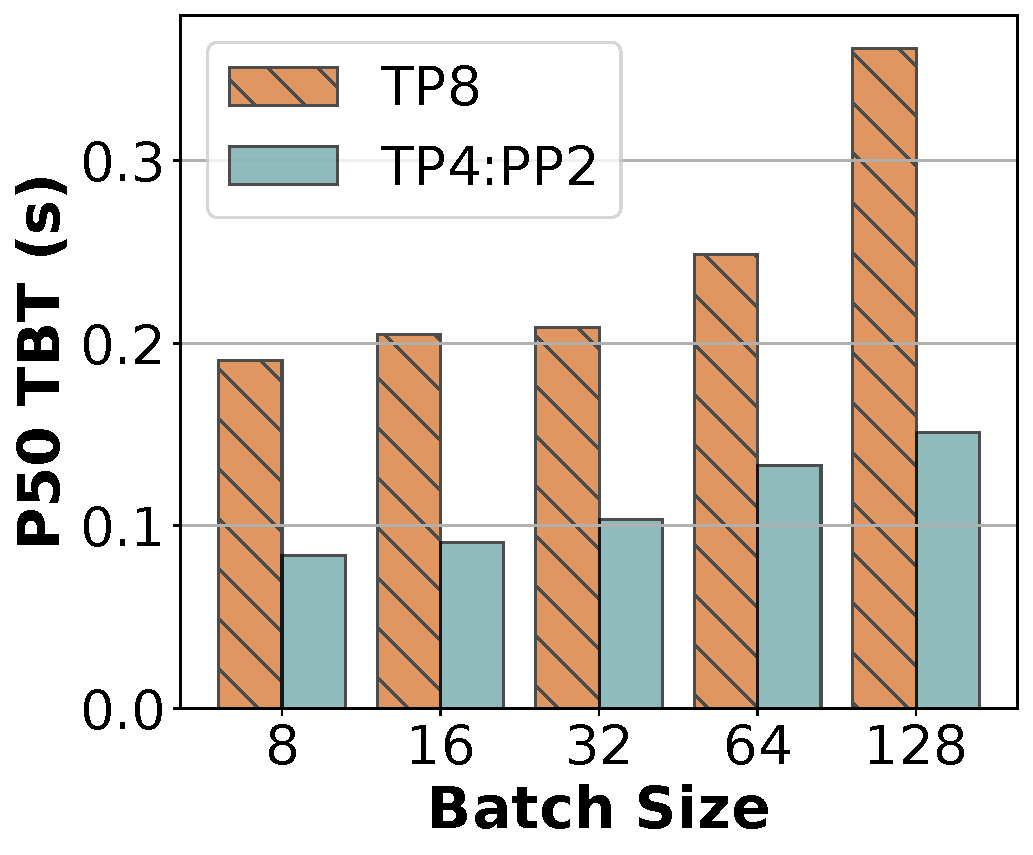
\includegraphics[width=\textwidth]{figures/pp-tp-latency.pdf}
    \caption{TBT (Falcon-180B).}
    \label{fig:eval:tp-latency}
\end{subfigure}
\begin{subfigure}{0.235\textwidth}
    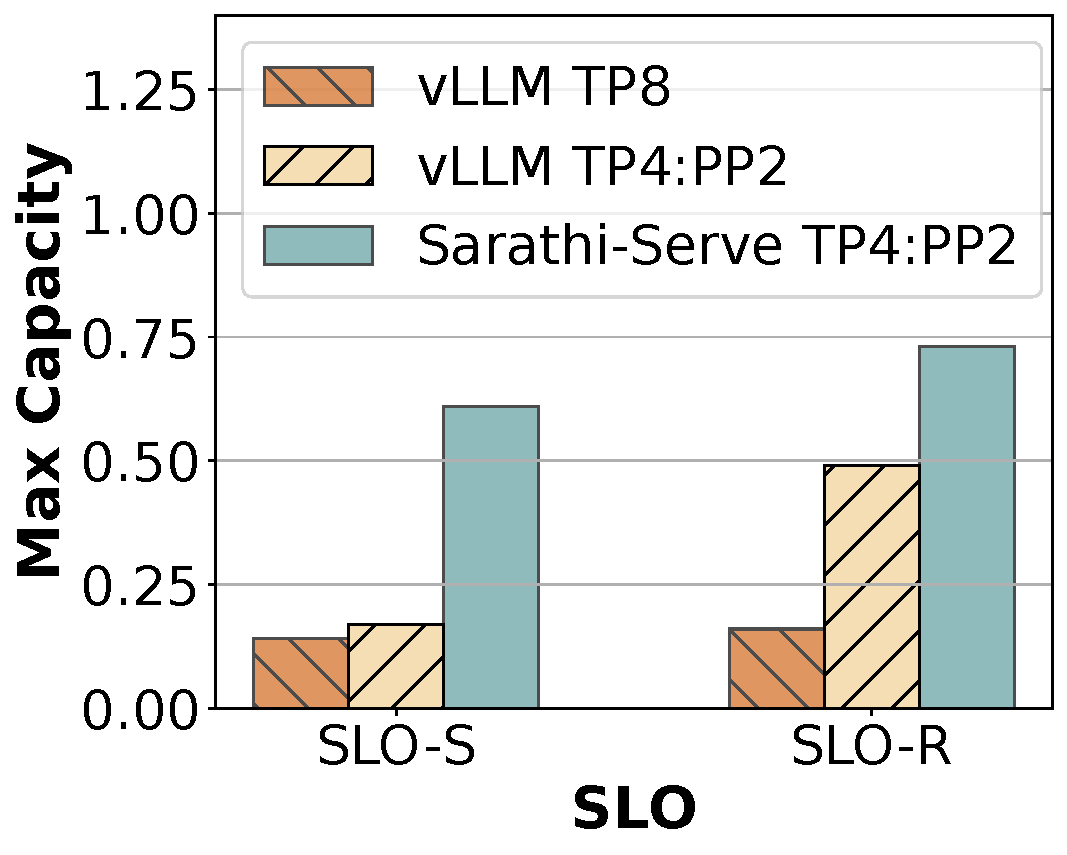
\includegraphics[width=\textwidth]{figures/pp-tp-capacity.pdf}
    \caption{Capacity (Falcon-180B).}
    \label{fig:eval:pp-tp-capacity}
\end{subfigure}
    \caption{TP scales poorly across nodes. (a) Median TBT for decode-only batches: cross node TP increases median TBT by more than $2\times$ compared to a 4-way TP within node and PP across nodes. (b) Capacity under strict (SLO-S) and
relaxed (SLO-R) latency SLOs: \sysname increases Falcon-180B's serving capacity by $4.3\times$ and $3.6\times$ over vLLM's TP-only and hybrid-parallel configurations under strict SLOs.}
    \label{fig:enter-label}
\end{figure}
